\documentclass[10pt]{beamer}

\usetheme{metropolis}
\usepackage{appendixnumberbeamer}
\usepackage[spanish]{babel}
\usepackage[utf8]{inputenc}
\usepackage[TS1,T1]{fontenc}
\usepackage{array}
\usepackage{graphicx}
\usepackage{colortbl}
\usepackage{caption}
\usepackage{subcaption}

\newcommand{\foo}{\color{gray}\makebox[0pt]{\textbullet}\hskip-0.5pt\vrule width 1pt\hspace{\labelsep}}

\usepackage{booktabs}
\usepackage[scale=2]{ccicons}

\usepackage{pgfplots}
\usepgfplotslibrary{dateplot}

\usepackage{multicol, multirow}

\usepackage{xspace}
\newcommand{\themename}{\textbf{\textsc{metropolis}}\xspace}

\title{Historia de los algoritmos inspirados en la evolución}
\subtitle{Algoritmos genéticos, programación evolutiva, estrategias de evolución y programación genética}
\date{\today}
\author{
  Francisco Luque Sánchez \\
  Ignacio Mas Mesa \\
  Miguel Morales Castillo \\
  María del Mar Ruiz Martín
}
\institute{Universidad de Granada}
% \titlegraphic{\hfill
\includegraphics[height=1.5cm]{logo.pdf}}

\begin{document}

\maketitle

\begin{frame}{Índice}
  \setbeamertemplate{section in toc}[sections numbered]
  \tableofcontents[hideallsubsections]
\end{frame}

\section{Introducción}

\begin{frame}[fragile]{Metaheurísticas}
  \begin{itemize}
  \item Aparecen en los años 50 (Optimización estocástica por Robbins y Monro) \\
  \item Resuelven problemas de optimización y búsqueda \\
  \item Tienen inspiraciones en procesos naturales \\
  \item Nos centraremos en las inspiradas en la evolución
  \end{itemize}
\end{frame}

\section{Programación evolutiva}

\begin{frame}[fragile]{Programación evolutiva}
  \begin{multicols}{2}
    ~\\
    \begin{itemize}
    \item Aparecen en 1964
    \item Su inventor es Lawrence J. Fogel
    \item Las utiliza para la predicción de series temporales
    \end{itemize}
    ~\\
    \begin{figure}[H]
      \centering
      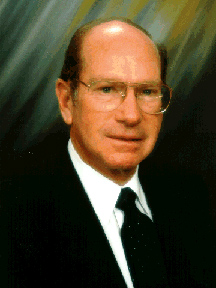
\includegraphics[scale=.5]{imgs/Fogel}
      \caption{Lawrence J. Fogel (\footnotesize{\url{http://ethw.org/w/images/7/7f/Fogel.jpg})}}
    \end{figure}
  \end{multicols}
\end{frame}

\begin{frame}{Primera propuesta}
  \begin{itemize}
  \item Representación de la línea temporal como cadena de símbolos
  \item Conjunto de autómatas finitos
  \item Evaluación de la capacidad de predicción
  \item Mutación de los autómatas (creación de la prole)
  \item Competición por la supervivencia (sobreviven los más aptos)
  \end{itemize}
\end{frame}

\begin{frame}{Evolución de la estrategia}
  \begin{table}
    \renewcommand\arraystretch{1.4}\arrayrulecolor{lightgray}
    \begin{tabular}{@{\,}r <{\hskip 2pt} !{\foo} >{\raggedright\arraybackslash}p{8cm}}
      \addlinespace[1.5ex]
      1969 & Aplicación a programas que juegan a juegos (Huntsinger)\\
      1980 & Nuevas representaciones de la solución (Fogel)\\
      1988 & Planificación de rutas (Fogel)\\
      1989 & Problema de la mochila (Fogel)\\
      1990 & Esquemas de adaptación de la evolución\\
      1992 & Aplicaciones en robótica (Donnel y Andersen)\\
      1995 & Diversificación del uso. Aplicación al entrenamiento de redes neuronales\\
    \end{tabular}
  \end{table}
\end{frame}

\section{Algoritmos genéticos}


\begin{frame}[fragile]{Algoritmos Genéticos}
    \begin{itemize}
    \item Surgen en 1962
    \item John Henry Holland (1929-2015)
    \item Interés en la evolución per sé
    \end{itemize}
\end{frame}




\begin{frame}[fragile]{Ciclo Evolutivo}
    \begin{figure}
    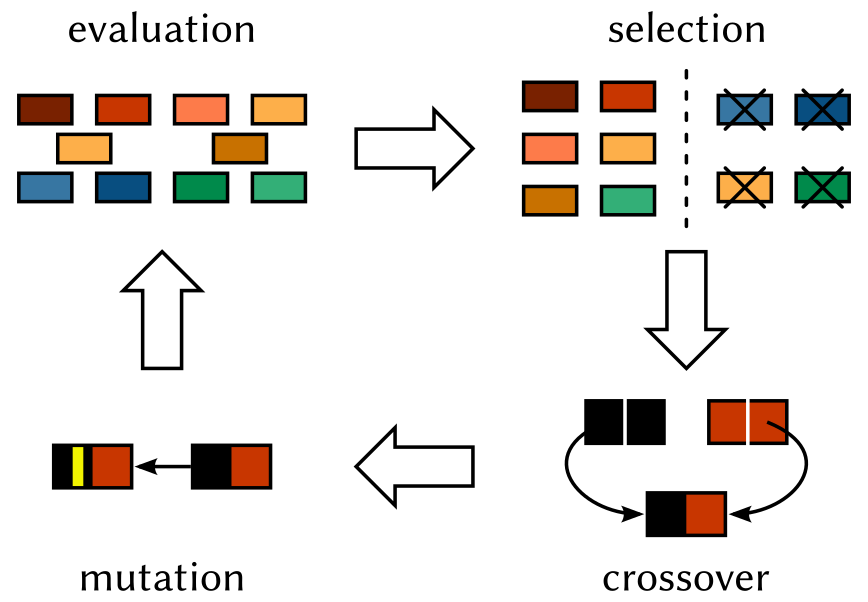
\includegraphics[scale=.34]{imgs/ciclo_evolucion_2_no_background}
      \caption*{\url{http://www.jade-cheng.com/au/coalhmm/optimization/}}
    \end{figure}
\end{frame}



\begin{frame}{Evolución de los Algoritmos Genéticos}
  \begin{table}
    \renewcommand\arraystretch{1.4}\arrayrulecolor{lightgray}
    \begin{tabular}{@{\,}r <{\hskip 2pt} !{\foo} >{\raggedright\arraybackslash}p{8cm}}
      \addlinespace[1.5ex]
      1962 & Nacen los Algoritmos Genéticos de mano de Holand\\
      1970's & Tesis de Bagley, Cavicchio y Frantz. Elitismo, mutación adaptativa y multicruce\\
      1975 & ``Adaptation in Natural and Artificial Systems'' (Holland)\\
           &  Teorema de los esquemas\\
           &  Tesis de Kenneth De Jong \\
      1980's & Aplicación en problemas de ingeniería y optimización\\
      1987 & ``Genetic Algorithms in Search, Optimization, and Machine Learning'' (Goldberg)\\
      1990's & Desaparición del operador de inversión y aplicación en problemas de ámbito real\\
    \end{tabular}
  \end{table}
\end{frame}

\begin{frame}{Evolución de la comunidad de los Algoritmos Genéticos}
  \begin{table}
    \renewcommand\arraystretch{1.4}\arrayrulecolor{lightgray}
    \begin{tabular}{@{\,}r <{\hskip 2pt} !{\foo} >{\raggedright\arraybackslash}p{8cm}}
      \addlinespace[1.5ex]
      1962 & Desarrollo en la Universidad de Míchigan\\
      1970's & Empiezan a surgir publicaciones: Bethke, Booker, Golberg\\
      1976 & Conferencia sobre Sistemas Adaptativos (Ann Arbor)\\
      1981 & ``An Interisciplinary Workshop in Adaptive Systems '' (Míchigan)\\
      1985 & Primera Conferencia Internacional de Algoritmos Genéticos (Pittsburgh)\\
      1989 & Creación de la Sociedad Internacional de Algoritmos Genéticos (ISGA)\\
    \end{tabular}
  \end{table}
\end{frame}



\section{Estrategias evolutivas}

\begin{frame}[fragile]{Autores}

  \begin{figure}[htp]
    \begin{subfigure}[b]{.3\textwidth}
      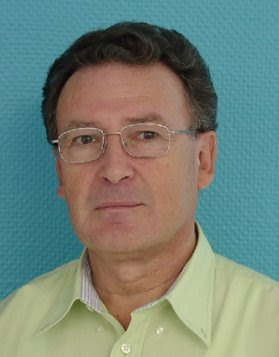
\includegraphics[width=.95\textwidth]{imgs/schwefel.jpg}
      \caption*{Hans-Paul Schwefel}
    \end{subfigure}%
    \begin{subfigure}[b]{.3\textwidth}
      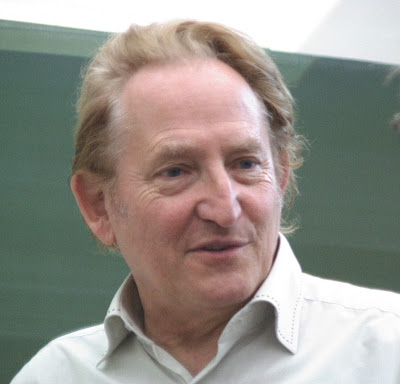
\includegraphics[width=.95\textwidth]{imgs/rechenberg.jpg}
      \caption*{Ingo Rechenberg}
    \end{subfigure}%
    \begin{subfigure}[b]{.3\textwidth}
      
\includegraphics[width=.95\textwidth]{imgs/bienert.jpg}
      \caption*{Peter Bienert}
    \end{subfigure}
  \end{figure}

\end{frame}

\begin{frame}{Experimento en túneles de viento}
  \begin{itemize}\itemsep2pt
  \item Técnicas clásicas
  \item Técnicas estocásticas
  \end{itemize}

  \begin{center}
    Nace la $(1 + 1)$ ES
  \end{center}
\end{frame}

\begin{frame}{Siguientes éxitos}
  \begin{itemize}\itemsep2pt
  \item Bienert construye un robot para automatizar los cálculos
  \item Lichtfu{\ss} diseña una tubería
  \item Diseño de una tobera supersónica
  \end{itemize}
\end{frame}

\begin{frame}{Inconvenientes}
  \begin{itemize}\itemsep2pt
  \item Distribuciones binomiales
  \item Convergencia prematura a óptimos locales
  \end{itemize}

  \begin{center}
    Distribuciones normales
  \end{center}
\end{frame}

\begin{frame}{Mejoras de Rechenberg}
  \begin{itemize}\itemsep2pt
  \item $\frac{1}{5}$ \emph{th rule}
  \item Recombinación y autoadaptación: $(\mu + 1)$ ES
  \end{itemize}
\end{frame}

\begin{frame}{Inconvenientes (II)}
  \begin{itemize}[<+- | alert@+>]
  \item Las $(\mu + 1)$ ES tenían poca capacidad de autoadaptación.
  \item Surgen las $\left( \mu \ \overset{+}{,} \ \lambda \right)$
  \end{itemize}
\end{frame}

\begin{frame}{Críticas}
  \begin{itemize}\itemsep2pt
  \item Gran avance de los métodos numéricos en la década pasada
  \item Críticas a $\mu > 1$ y $\lambda > 1$
  \item Críticas a $(\mu, \lambda)$
  \end{itemize}
\end{frame}

\section{Programación genética}

\begin{frame}{Programación genética}

 \begin{itemize}\itemsep2pt
  \item Richard Forsyth demuestra el éxito en la evolución de pequeños programas
  \item En 1988, John Koza patenta un algoritmo genético orientado a la evolución de programas
  \item John Koza se considera el mayor exponente de la programación genética
  \item Se aplica a problemas sencillos por el alto coste computacional
  \end{itemize}
  
\end{frame}

\begin{frame}{Algoritmo planteado}

 \begin{figure}[H]
  \centering
  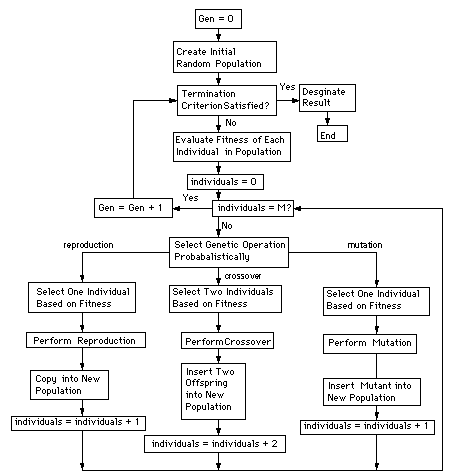
\includegraphics[width=0.7\textwidth]{imgs/FlowchartGP.PNG}
  \label{fig:dfd:1}
\end{figure}
  
\end{frame}


\begin{frame}{Conclusión}

 \begin{itemize}\itemsep2pt
  \item Estrategias muy parecidas debido a la falta de comunicación
  \item Gran importancia en la ciencia de la computación pese al escepticismo inicial
  \item El aumento de los recursos y la capacidad de cómputo en el futuro ampliará el abanico de aplicaciones posibles.
  \end{itemize}

  
\end{frame}

\begin{frame}[standout]
  ¿Preguntas?
\end{frame}

\end{document}
